\documentclass[11pt,a4paper]{article}
\usepackage[T1]{fontenc}
\usepackage[utf8]{inputenc}
\usepackage{lmodern}
\usepackage[brazil]{babel}
\usepackage[margin=2cm]{geometry}
\usepackage{amsmath,amssymb}
\usepackage{booktabs}
\usepackage{enumitem}
\usepackage{caption}
\usepackage{graphicx}
\usepackage{placeins}
\usepackage{microtype}
\usepackage[compact]{titlesec}
\usepackage[hidelinks]{hyperref}

% figuras geradas por graficos/gera_graficos.py (raiz do repositorio)
\graphicspath{{../../graficos/}}

\titlespacing*{\section}{0pt}{1.0em}{0.4em}
\captionsetup{font=small,labelfont=bf}
\setlist{nosep,leftmargin=1.4em}
\setlength{\parskip}{0.35em}
\pagestyle{plain}
\renewcommand{\topfraction}{0.9}
\renewcommand{\textfraction}{0.07}
\renewcommand{\floatpagefraction}{0.85}

\newcommand{\cmax}{C_{\max}}

\begin{document}

\noindent{\LARGE\bfseries Otimização do Sequenciamento na Produção de Baterias:\\[2pt] Abordagem via RCPSP}\\[6pt]
{\bfseries Etapas 5 e 6: Resultados dos Métodos Exato e Aproximado}\\
Cristian Madeira (Pós), Otávio Novais (162962), Thaís Melo (164934)

\section{Objetivo}

Este relatório reúne os resultados das Etapas~5 e~6. O sequenciamento das atividades na produção
de baterias foi modelado como um RCPSP (\emph{resource-constrained project scheduling problem}):
minimizar o makespan $\cmax$ respeitando as precedências e a capacidade dos recursos renováveis.
O problema foi resolvido de duas formas, nas mesmas instâncias: por um modelo exato de programação
linear inteira mista (Gurobi) e pela metaheurística RKO (\emph{Random-Key Optimizer}). A
comparação procura responder a três perguntas:
\begin{enumerate}
  \item Até que tamanho de instância o método exato entrega o ótimo com prova, e por que falha
        quando não entrega? (Seção~\ref{sec:exato})
  \item Quanto se ganha, em tempo e em qualidade, ao trocar o método exato pelo aproximado?
        (Seção~\ref{sec:comparacao})
  \item Dentro do método aproximado, o que mais importa: a estratégia de busca (GA, BRKGA ou RKO)
        ou o decodificador? (Seção~\ref{sec:busca})
\end{enumerate}

\section{Instâncias e configuração}

\textbf{Instâncias.} Foram usadas 15 instâncias da PSPLIB \cite{psplib}, todas com quatro recursos
e ótimo $C^*$ conhecido:
\begin{itemize}
  \item dez do J30 (30 atividades): j301\_1, a instância apresentada na Etapa~3, e nove dos grupos
        mais difíceis, uma por grupo, todas com recursos escassos ($RS = 0{,}2$ ou $0{,}5$);
  \item cinco do J60 (60 atividades), com $RS = 0{,}2$, acrescentadas na Etapa~6 para avaliar o
        efeito do tamanho.
\end{itemize}
Os ótimos de referência foram obtidos com o CP-SAT (OR-Tools), com otimalidade provada. Nos grupos
com $RS \ge 0{,}7$, o ótimo praticamente coincide com o limitante trivial (caminho crítico ou carga
de recurso), e os métodos não se diferenciam; por isso, essas instâncias não foram usadas. Todos os
experimentos rodaram no mesmo notebook (Intel Core i5-1135G7, 16~GB de RAM, Linux).

\textbf{Método exato.} Modelo tempo-indexado de Pritsker et al.\ \cite{pritsker}, em AMPL,
resolvido pelo Gurobi~13.0.3 com limite de 600~s por instância. Em relação à formulação da
Etapa~4, foram adotados três refinamentos que não alteram o conjunto de soluções ótimas:
\begin{itemize}
  \item \textbf{precedência desagregada}: $\sum_{s \le t} x_{js} \le \sum_{s \le t-p_i} x_{is}$ para
        cada arco $(i,j)$ e período $t$ \cite{christofides};
  \item \textbf{horizonte e janelas}: $H$ é o melhor makespan do SSGS com sete regras de prioridade
        seguido de \emph{forward-backward improvement} (FBI) \cite{valls}; a variável $x_{jt}$ só
        existe para $t \in [ES_j, LS_j]$;
  \item \textbf{solução inicial}: o cronograma heurístico que define $H$ é dado ao solver.
\end{itemize}
Cada solução devolvida foi conferida por uma rotina independente do modelo (precedência, capacidade
e makespan), e todas foram aprovadas.

\textbf{Método aproximado.} RKO \cite{rko}, na implementação C++ dos autores, sem alterações nas
metaheurísticas. O decodificador é próprio do RCPSP: o vetor de chaves gera uma lista de prioridade
topologicamente válida (a cada passo, a atividade elegível de menor chave), que o SSGS converte em
cronograma e o FBI melhora. O RKO executa nove metaheurísticas em paralelo (BRKGA, SA, GRASP, ILS,
VNS, PSO, GA, LNS e BRKGA-CS), que compartilham um conjunto de soluções de elite. Foram usados dois
critérios de parada, ambos com 10 execuções por instância e encerramento ao atingir $C^*$:
\begin{itemize}
  \item \textbf{tempo}: 10~s por execução no J30 e 30~s no J60;
  \item \textbf{orçamento}: 50.000 cronogramas (decodificações, somadas entre as threads), o
        critério usual da literatura \cite{kolisch}.
\end{itemize}
Para separar o efeito da estratégia de busca, o GA e o BRKGA \cite{brkga} do mesmo framework também
foram executados isoladamente, com o mesmo decodificador, com e sem o FBI.

\textbf{Métrica.} A qualidade é medida pelo desvio relativo ao ótimo,
RPD $= 100\,(\cmax - C^*)/C^*$. RPD $= 0$ significa que o ótimo foi encontrado.

\section{Método exato}\label{sec:exato}

\begin{table}[!htbp]
\centering
\small
\setlength{\tabcolsep}{4.6pt}
\caption{Modelo tempo-indexado no Gurobi (600~s por instância).}
\label{tab:exato}
\begin{tabular}{lccrrrrrrcr}
\toprule
Instância & $RF$ & $RS$ & Binárias & $H$ & LP & $\cmax$ & LB & $C^*$ & Status & Tempo (s) \\
\midrule
% valores de results/exact_selecao_j30_gurobi_D.csv e results/exact_selecao_j60_gurobi_D.csv
j301\_1   & 0,25 & 0,2 &   482 &  46 &  38,8 & \textbf{43}  &  43 &  43 & ótimo  &   0,1 \\
j309\_2   & 0,75 & 0,2 & 1.879 &  98 &  63,0 & \textbf{92}  &  92 &  92 & ótimo  & 286,5 \\
j3013\_1  & 1,00 & 0,2 & 1.061 &  64 &  48,3 & 59           &  53 &  58 & limite & 600,1 \\
j3025\_4  & 0,75 & 0,2 & 1.515 &  89 &  55,3 & \textbf{81}  &  81 &  81 & ótimo  & 242,8 \\
j3029\_8  & 1,00 & 0,2 & 1.454 &  89 &  66,5 & 81           &  72 &  80 & limite & 600,1 \\
j3037\_7  & 0,50 & 0,2 & 1.603 &  98 &  58,3 & \textbf{92}  &  92 &  92 & ótimo  &  40,9 \\
j3041\_10 & 0,75 & 0,2 & 1.740 & 106 &  69,4 & \textbf{99}  &  99 &  99 & ótimo  & 165,7 \\
j3045\_6  & 1,00 & 0,2 & 2.290 & 133 &  89,1 & \textbf{129} & 124 & 129 & limite & 600,1 \\
j3014\_2  & 1,00 & 0,5 &   599 &  56 &  46,8 & \textbf{53}  &  53 &  53 & ótimo  &  51,0 \\
j3030\_2  & 1,00 & 0,5 &   663 &  70 &  65,0 & \textbf{68}  &  68 &  68 & ótimo  &   6,0 \\
\midrule
j605\_4   & 0,50 & 0,2 & 2.700 &  83 &  58,3 & 77           &  66 &  72 & limite & 600,1 \\
j609\_4   & 0,75 & 0,2 & 2.821 &  94 &  72,9 & 92           &  83 &  87 & limite & 600,1 \\
j6021\_4  & 0,50 & 0,2 & 3.344 & 109 &  73,0 & 96           &  90 &  95 & limite & 600,1 \\
j6037\_2  & 0,50 & 0,2 & 2.673 & 100 &  72,3 & 96           &  88 &  95 & limite & 600,1 \\
j6041\_7  & 0,75 & 0,2 & 4.872 & 152 & 109,2 & 147          & 124 & 132 & limite & 600,2 \\
\bottomrule
\end{tabular}
\par\smallskip
\begin{minipage}{0.97\textwidth}\footnotesize
$RF$, $RS$: fator e força de recurso do gerador ProGen. $H$: horizonte (heurística). LP: relaxação
linear. $\cmax$: melhor solução inteira (em negrito quando igual a $C^*$). LB: melhor limitante
inferior. Status: ótimo provado ou limite de tempo atingido.
\end{minipage}
\end{table}

\begin{figure}[!htbp]
\centering
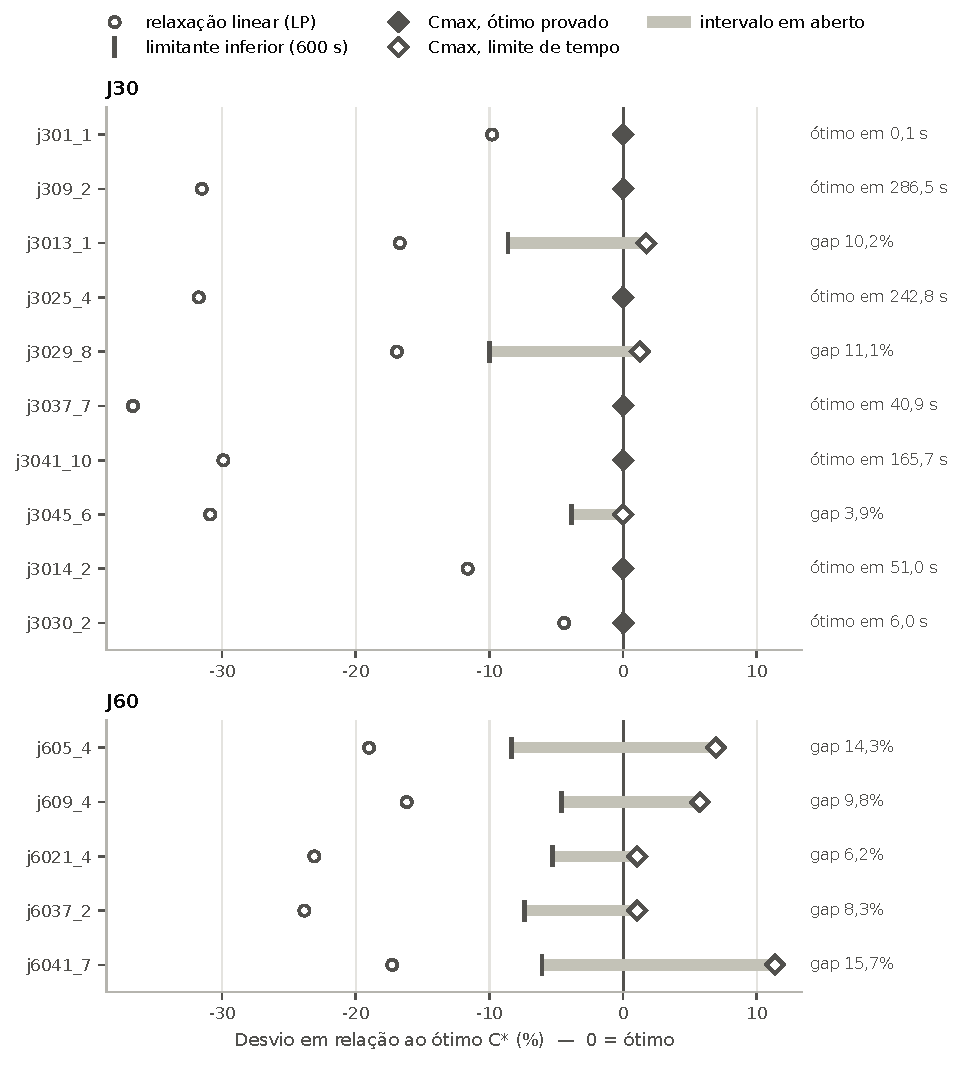
\includegraphics[width=0.64\textwidth]{fig4_gap_gurobi}
\caption{Posição da relaxação linear, do limitante inferior e da melhor solução do Gurobi em relação
ao ótimo ($C^* = 0$). A barra cinza é o intervalo que o solver não fechou em 600~s; à direita, o
gap final ou o tempo até a prova de otimalidade.}
\label{fig:gap}
\end{figure}

\textbf{J30: ótimo com prova na maioria das instâncias.} O Gurobi provou a otimalidade em 7 das 10
instâncias, entre 0,1~s e 287~s (Tabela~\ref{tab:exato}). Nas outras três, as soluções continuam
boas: em j3045\_6, o solver encontrou o ótimo (129), mas não o provou; em j3013\_1 e j3029\_8, terminou
uma unidade acima do ótimo. O RPD médio no J30 é de 0,30\%.

\textbf{J60: nenhuma prova em 600~s.} Nas cinco instâncias J60, o limite de tempo foi atingido, com
gap entre 6,2\% e 15,7\% e RPD médio de 5,2\%. O modelo tem de 2.700 a 4.900 binárias, contra 480 a
2.300 no J30, porque o número de variáveis acompanha o produto entre o número de atividades e o
horizonte.

\textbf{O tipo de dificuldade muda com o tamanho.} A Figura~\ref{fig:gap} mostra de que lado do
ótimo fica o intervalo em aberto. Nas três J30 não resolvidas, a solução está no ótimo ou a no
máximo 1,7\% dele, e quase todo o gap vem do limitante inferior (de 3,9\% a 10\% abaixo de $C^*$): o
solver já tem a resposta, mas não consegue prová-la. No J60, o lado das soluções também falha: em
j605\_4 e j6041\_7, a melhor solução fica 6,9\% e 11,4\% acima do ótimo, um erro maior que o do
limitante (8,3\% e 6,1\% abaixo). Ou seja, nas instâncias maiores, o método exato tem dificuldade
até para encontrar boas soluções.

\textbf{Relaxação linear fraca.} A relaxação linear fica, em média, 22\% abaixo do ótimo no J30 e
20\% no J60, e o solver precisa enumerar muitos nós para fechar essa distância. A fraqueza da
relaxação, porém, não explica sozinha a dificuldade: j3037\_7, com a pior relaxação (37\% abaixo),
foi resolvida em 41~s, enquanto j3013\_1 (17\% abaixo) não foi. As três J30 não resolvidas são
exatamente as de $RF = 1{,}0$ e $RS = 0{,}2$, em que todas as atividades usam os quatro recursos e
esses recursos são escassos, o que multiplica os conflitos de capacidade.

\textbf{Papel da heurística.} O horizonte $H$ ficou, em média, 7\% acima do ótimo no J30 e 12\% no
J60. O Gurobi melhorou essa solução inicial em todas as 15 instâncias, de modo que o método exato
agrega valor sobre a heurística construtiva, mesmo quando não prova a otimalidade.

\section{Exato \texorpdfstring{$\times$}{x} aproximado}\label{sec:comparacao}

\begin{figure}[!htbp]
\centering
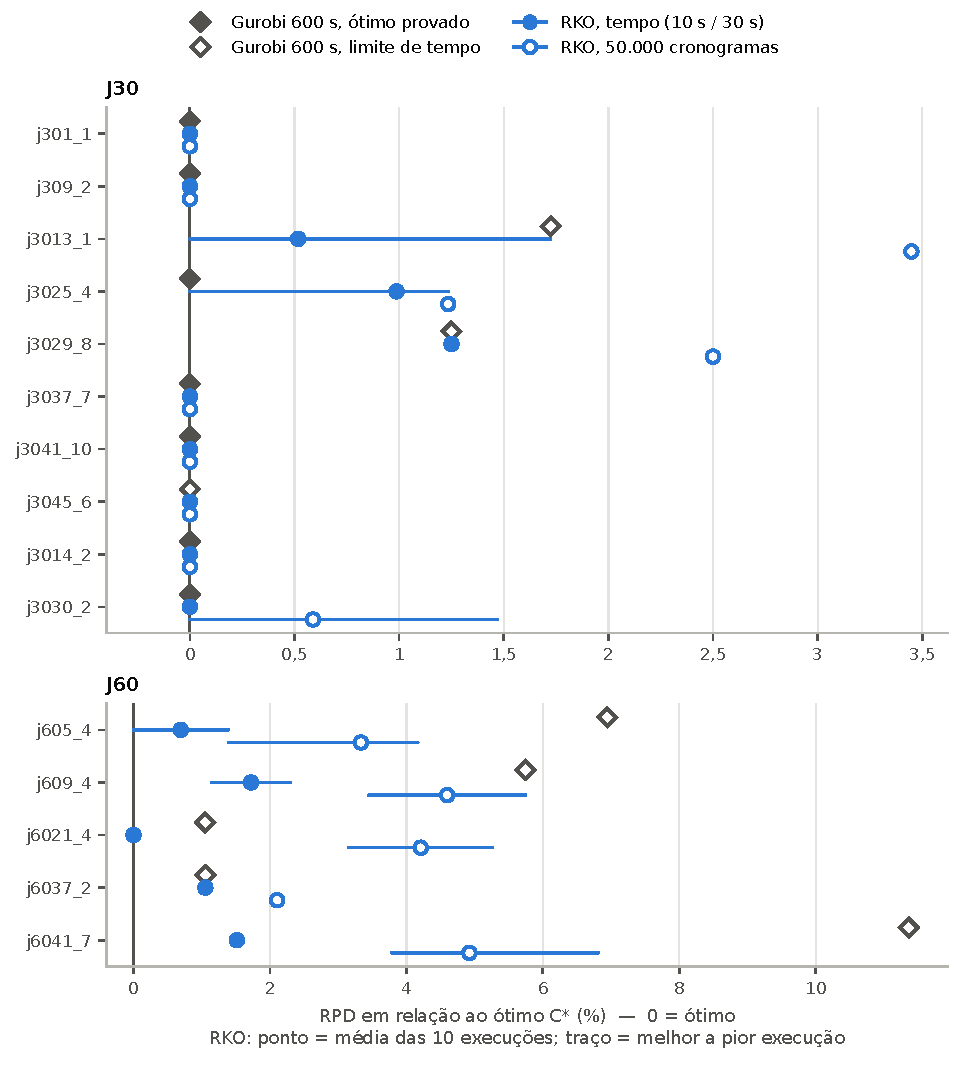
\includegraphics[width=0.64\textwidth]{fig1_exato_rko}
\caption{RPD por instância do Gurobi (600~s) e do RKO nos dois critérios de parada. RKO: média das
10 execuções (ponto) e intervalo entre a melhor e a pior execução (traço). Os eixos dos dois
painéis têm escalas diferentes.}
\label{fig:instancias}
\end{figure}

\textbf{Por instância.} A Figura~\ref{fig:instancias} compara os métodos instância a instância.
\begin{itemize}
  \item \textbf{J30.} Seis das dez instâncias são resolvidas por todos os métodos, em todas as
        execuções. Nas demais, o RKO com tempo atinge o ótimo em j3013\_1 (o Gurobi parou em 59),
        empata com o Gurobi em j3029\_8 (81, uma unidade acima do ótimo, que nenhum método
        alcançou), empata em j3030\_2 (ambos no ótimo) e fica atrás em j3025\_4 (média de 81,8
        contra o ótimo provado do Gurobi). Com
        50.000 cronogramas, o RKO fica atrás do Gurobi nas quatro instâncias não triviais.
  \item \textbf{J60.} O RKO com tempo é melhor que o Gurobi em quatro instâncias e empata em
        j6037\_2. Em j6041\_7, a diferença é de 1,5\% contra 11,4\%. Mesmo com 50.000 cronogramas,
        o RKO supera o Gurobi em três das cinco instâncias.
\end{itemize}
Os traços mostram que a variação entre execuções do RKO é pequena com o critério de tempo (no
máximo 1,7 ponto percentual entre a melhor e a pior execução) e maior com o orçamento fixo (até
3 pontos no J60).

\begin{figure}[!htbp]
\centering
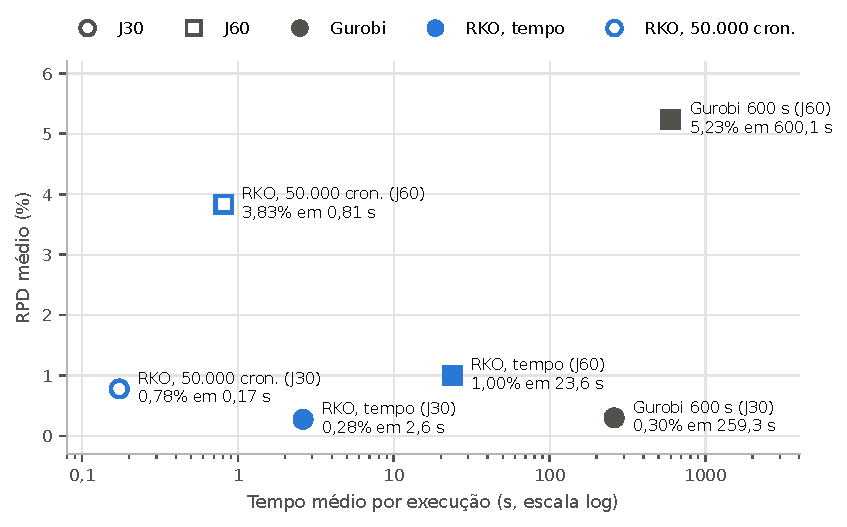
\includegraphics[width=0.85\textwidth]{fig2_qualidade_tempo}
\caption{RPD médio $\times$ tempo médio por execução (escala logarítmica), por conjunto de
instâncias. Pontos mais próximos do canto inferior esquerdo são melhores nos dois critérios.}
\label{fig:qualidade-tempo}
\end{figure}

\textbf{Qualidade e tempo.} A Figura~\ref{fig:qualidade-tempo} resume o compromisso entre os dois
critérios:
\begin{itemize}
  \item \textbf{No J30, a qualidade é a mesma, mas o RKO é cerca de 100 vezes mais rápido}: 0,28\% em
        2,6~s, contra 0,30\% em 259~s do Gurobi. A vantagem que resta ao método exato é a prova de
        otimalidade, obtida em 7 das 10 instâncias.
  \item \textbf{No J60, o RKO é melhor nos dois critérios}: 1,0\% em 24~s, contra 5,2\% em 600~s.
  \item \textbf{O orçamento de 50.000 cronogramas} é o ponto mais rápido (menos de 1~s), ao custo de
        qualidade: 0,78\% no J30 e 3,8\% no J60, ainda melhor que o Gurobi neste último.
\end{itemize}
Em nenhum dos dois conjuntos o Gurobi é a melhor opção quando o objetivo é apenas uma boa solução:
o RKO com tempo é igual ou melhor em qualidade e de 25 a 100 vezes mais rápido. A vantagem do
método aproximado cresce com o tamanho da instância, de acordo com o que se viu na
Seção~\ref{sec:exato}.

\section{Estratégia de busca e decodificador}\label{sec:busca}

\begin{figure}[!htbp]
\centering
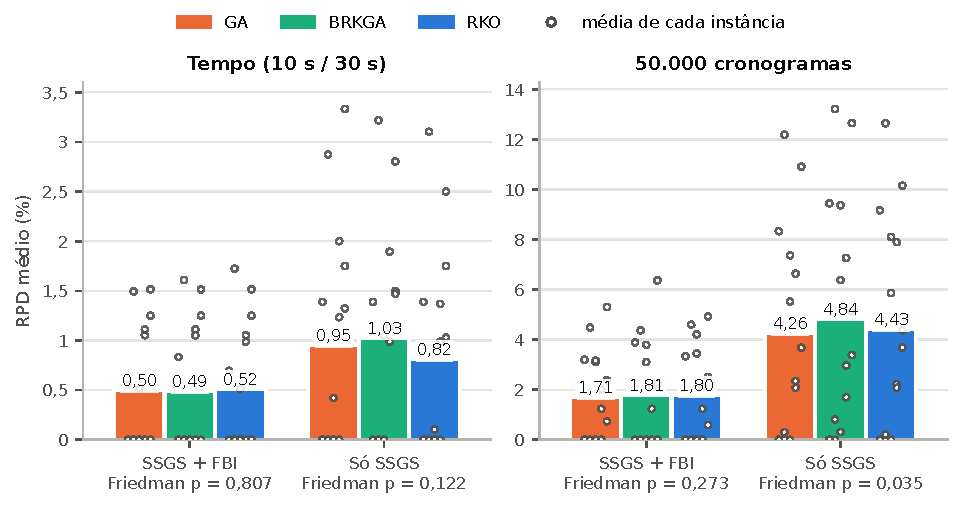
\includegraphics[width=0.9\textwidth]{fig3_estrategias_busca}
\caption{RPD médio nas 15 instâncias (10 execuções cada) do GA, do BRKGA e do RKO, com e sem o FBI
no decodificador, nos dois critérios de parada. Os pontos são o RPD médio de cada instância; abaixo
de cada grupo, o $p$ do teste de Friedman entre os três métodos.}
\label{fig:busca}
\end{figure}

Para avaliar a observação de que algoritmos genéticos têm dificuldade neste problema, o GA e o BRKGA
foram comparados ao RKO com a mesma representação e o mesmo decodificador
(Figura~\ref{fig:busca}).

\textbf{A estratégia de busca pouco importa.} Com o FBI, os três métodos são estatisticamente
equivalentes nos dois critérios (Friedman: $p = 0{,}81$ com tempo e $p = 0{,}27$ com orçamento).
A única diferença significativa aparece sem o FBI e com orçamento fixo ($p = 0{,}035$): o GA supera o
BRKGA (Wilcoxon pareado com correção de Holm, $p = 0{,}02$), e o RKO fica entre os dois. Os pontos da
figura reforçam a conclusão: a diferença entre instâncias (de 0 a 13\% de RPD) é muito maior que a
diferença entre métodos (menos de 0,6 ponto percentual). A dificuldade esperada do GA, portanto,
não se confirmou. Uma explicação provável para o desempenho inferior do BRKGA sem FBI é o
orçamento: o framework divide os cronogramas entre nove cópias paralelas, e, com a população padrão
de 987 indivíduos, cada cópia do BRKGA faz só 3 a 4 gerações, contra 8 a 11 do GA (população de 400).

\textbf{O decodificador é o fator de maior efeito.} O FBI reduz o RPD médio de 4,3--4,8\% para
1,7--1,8\% com orçamento fixo e de 0,8--1,0\% para cerca de 0,5\% com tempo. Há uma ressalva na
comparação por orçamento: com o FBI, cada cronograma contado envolve, em média, 5,3 a 5,6 passadas
do SSGS (a original e as de justificação), e por isso o FBI avalia cerca de 5 vezes menos
cronogramas por segundo (90 mil contra 500 mil). A comparação por tempo, que desconta esse custo,
mantém a conclusão: mesmo avaliando menos cronogramas, o FBI reduz o RPD no J60 de 1,7--2,1\% para
0,9--1,0\% (Mann-Whitney, $p < 0{,}01$ nos três métodos). No J30, a diferença é pequena
(0,24--0,29\% contra 0,38--0,51\%), porque a maioria das execuções já chega ao ótimo.

\FloatBarrier
\section{Limitações}

\begin{itemize}
  \item Foram usadas 15 instâncias, escolhidas entre as de recursos escassos. Os resultados não se
        estendem diretamente às instâncias fáceis ($RS \ge 0{,}7$) nem ao J90 e ao J120.
  \item Os parâmetros das metaheurísticas são os padrão do framework e não foram calibrados para o
        orçamento de 50.000 cronogramas, o que limita a comparação entre GA e BRKGA.
  \item Os tempos foram medidos em uma única máquina, e os dois métodos usam paralelismo de formas
        diferentes (o RKO, nove metaheurísticas em threads separadas; o Gurobi, o
        \emph{branch-and-bound} paralelo), o que torna a razão entre os tempos apenas indicativa.
\end{itemize}

\section{Conclusões}

\begin{itemize}
  \item \textbf{Instâncias pequenas (J30):} o modelo exato entrega o ótimo com prova em 7 de 10
        instâncias, a um custo de minutos. Quando falha, a solução é boa e o que falta é a prova
        (limitante inferior fraco nas instâncias com $RF = 1{,}0$ e $RS = 0{,}2$).
  \item \textbf{Instâncias maiores (J60):} o modelo exato não prova nenhum ótimo em 600~s e passa a
        errar também nas soluções (RPD médio de 5,2\%). O RKO obtém 1,0\% em 24~s.
  \item \textbf{Metaheurística:} com o mesmo decodificador, GA, BRKGA e RKO são equivalentes; o que
        decide a qualidade é o FBI no decodificador.
\end{itemize}
Os dois métodos são complementares. O RKO é a escolha para gerar boas soluções rapidamente, e o
método exato, para certificar o ótimo em instâncias pequenas. Uma combinação natural para o
artigo é usar a solução do RKO como horizonte e solução inicial do modelo exato: um $H$ mais
justo estreita as janelas $[ES_j, LS_j]$ e reduz o número de binárias, o que pode tornar o J60
tratável pelo Gurobi. O RKO será a metaheurística do artigo, com o GA e o BRKGA como referência.

\vspace{-0.4em}
{\footnotesize
\renewcommand{\refname}{\normalsize Referências}
\begin{thebibliography}{9}\setlength{\itemsep}{0pt}
\bibitem{rko} Chaves, A. A. et al. A random-key optimizer for combinatorial optimization. \emph{Journal of Heuristics}, 31(4), 2025.
\bibitem{christofides} Christofides, N.; Alvarez-Valdés, R.; Tamarit, J. M. Project scheduling with resource constraints: a branch and bound approach. \emph{European Journal of Operational Research}, 29(3):262--273, 1987.
\bibitem{brkga} Gonçalves, J. F.; Resende, M. G. C. Biased random-key genetic algorithms for combinatorial optimization. \emph{Journal of Heuristics}, 17(5):487--525, 2011.
\bibitem{kolisch} Kolisch, R.; Hartmann, S. Experimental investigation of heuristics for resource-constrained project scheduling: an update. \emph{European Journal of Operational Research}, 174(1):23--37, 2006.
\bibitem{psplib} Kolisch, R.; Sprecher, A. PSPLIB -- a project scheduling problem library. \emph{European Journal of Operational Research}, 96(1):205--216, 1997.
\bibitem{pritsker} Pritsker, A. A. B.; Watters, L. J.; Wolfe, P. M. Multiproject scheduling with limited resources: a zero-one programming approach. \emph{Management Science}, 16(1):93--108, 1969.
\bibitem{valls} Valls, V.; Ballestín, F.; Quintanilla, S. Justification and RCPSP: a technique that pays. \emph{European Journal of Operational Research}, 165(2):375--386, 2005.
\end{thebibliography}}

\end{document}
